\documentclass{article}
\setlength{\headheight}{36pt}
\addtolength{\topmargin}{-24pt}
\usepackage{indentfirst}
\usepackage{fancyhdr}
\usepackage{amsmath}
\usepackage{amssymb}
\usepackage{graphicx}
\usepackage[margin=1in]{geometry}
\usepackage{hyperref}
\usepackage[T1]{fontenc}
\usepackage[utf8]{inputenc}
\usepackage{xcolor}
\usepackage{listings}
\usepackage{listingsutf8}

% Estilo para códigos em Python
\lstset{
  language=Python,
  inputencoding=utf8/latin1,
  extendedchars=true,
  basicstyle=\ttfamily\small,
  keywordstyle=\color{blue!70!black},
  commentstyle=\color{teal!70!black},
  stringstyle=\color{orange!60!black},
  showstringspaces=false,
  columns=fullflexible,
  numbers=left,
  numberstyle=\tiny,
  stepnumber=1,
  numbersep=8pt,
  frame=single,
  breaklines=true,
  tabsize=4,
  captionpos=b
}
\usepackage[portuguese]{babel}
\usepackage{textcomp}

\title{Resolução da Lista de Exercícios}
\author{\textbf{Francisco Davi Belo Rodrigues}}
\date{\today}

\begin{document}

\fancyhead{}
\fancyhead[C]{%
  {\large\textbf{Universidade Federal do Rio de Janeiro}}\\
  {\normalsize Programa de Pós-Graduação em Engenharia de Processos Químicos e Bioquímicos} \\
  {\normalsize Disciplina EQE 776 - Modelagem e Simulação de Processos}
}

\maketitle
\thispagestyle{fancy}

\section{Exercício 1}

\subsection*{Enunciado e dados}
Consideram-se dois tanques cilíndricos interligados em série. O tanque 1 recebe uma alimentação constante e descarrega no tanque 2, que por sua vez escoa para o ambiente. As vazões de saída de cada tanque dependem do nível interno segundo a relação empírica $Q_i = k_i\sqrt{h_i}$. Os parâmetros fornecidos são resumidos na Tabela~\ref{tab:dados-q1}.

\begin{table}[h!]
  \centering
  \begin{tabular}{ll}
    \hline
    \textbf{Parâmetro} & \textbf{Valor} \\
    \hline
    Vazão de alimentação $Q_0$ & $20\ \mathrm{m^3\,h^{-1}}$ \\
    Diâmetro do tanque 1 $D_1$ & $4\ \mathrm{m}$ \\
    Diâmetro do tanque 2 $D_2$ & $3\ \mathrm{m}$ \\
    Constante da válvula 1 $k_1$ & $14\ \mathrm{m^{2.5}\,h^{-1}}$ \\
    Constante da válvula 2 $k_2$ & $12\ \mathrm{m^{2.5}\,h^{-1}}$ \\
    Nível inicial no tanque 1 $h_1(0)$ & $3\ \mathrm{m}$ \\
    Nível inicial no tanque 2 $h_2(0)$ & $2\ \mathrm{m}$ \\
    \hline
  \end{tabular}
  \caption{Dados operacionais da Questão 1.}
  \label{tab:dados-q1}
\end{table}

\subsection*{Formulação do modelo}

O modelo dinâmico é obtido a partir dos balanços de massa (ou volume, dado que a densidade é constante) em cada tanque. Para um volume de controle genérico com densidade constante $\rho$, tem-se
\begin{equation*}
  \frac{d(\rho V)}{dt} = \rho Q_{\text{in}} - \rho Q_{\text{out}},
\end{equation*}
o que conduz ao balanço volumétrico
\begin{equation*}
  \frac{dV}{dt} = Q_{\text{in}} - Q_{\text{out}}.
\end{equation*}

No tanque 1, o volume contido é $V_1 = A_1 h_1$, com $A_1$ indicado na Eq.~\eqref{eq:area1}. O balanço volumétrico resulta em
\begin{equation*}
  A_1\,\frac{dh_1}{dt} = Q_0 - Q_1,
\end{equation*}
em que $Q_0$ é a vazão de alimentação e $Q_1$ a vazão de saída do tanque 1. De modo análogo, para o tanque 2 obtém-se $V_2 = A_2 h_2$ e
\begin{equation*}
  A_2\,\frac{dh_2}{dt} = Q_1 - Q_2,
\end{equation*}
com $Q_1$ proveniente do tanque 1 e $Q_2$ a descarga para o ambiente.

As vazões de saída seguem a correlação empírica das válvulas e as áreas dos tanques são calculadas pela geometria cilíndrica. Mantendo $t$ em horas, têm-se as equações numeradas finais:
\begin{align}
  A_i &= \frac{\pi D_i^2}{4}, \quad i = 1,2, \label{eq:area1} \\
  Q_1 &= k_1 \sqrt{h_1}, \label{eq:Q1} \\
  Q_2 &= k_2 \sqrt{h_2}, \label{eq:Q2} \\
  A_1\,\frac{dh_1}{dt} &= Q_0 - Q_1, \label{eq:balanco1} \\
  A_2\,\frac{dh_2}{dt} &= Q_1 - Q_2, \label{eq:balanco2}
\end{align}
com condições iniciais $h_1(0) = 3\ \mathrm{m}$ e $h_2(0) = 2\ \mathrm{m}$. Este conjunto de equações está pronto para utilização em ambientes de simulação como o EMSO, onde os parâmetros podem ser definidos separadamente sem substituição numérica antecipada.

\subsection*{Resolução numérica}
O sistema diferencial foi integrado em $0 \leq t \leq 20\ \mathrm{h}$ empregando o método Runge--Kutta de quarta/quinta ordem adaptativo (\texttt{solve\_ivp} do SciPy) com passo máximo equivalente a $10\ \mathrm{s}$ após conversão interna de unidades no script de apoio. A implementação registra também as trajetórias discretizadas $(t, h_1, h_2)$ em arquivo auxiliar para rastreabilidade.

\lstinputlisting[caption={Script Python utilizado para a integracao numerica da Questao 1.},label={lst:python-q1}]{solucao_questao1.py}

\begin{figure}[h!]
  \centering
  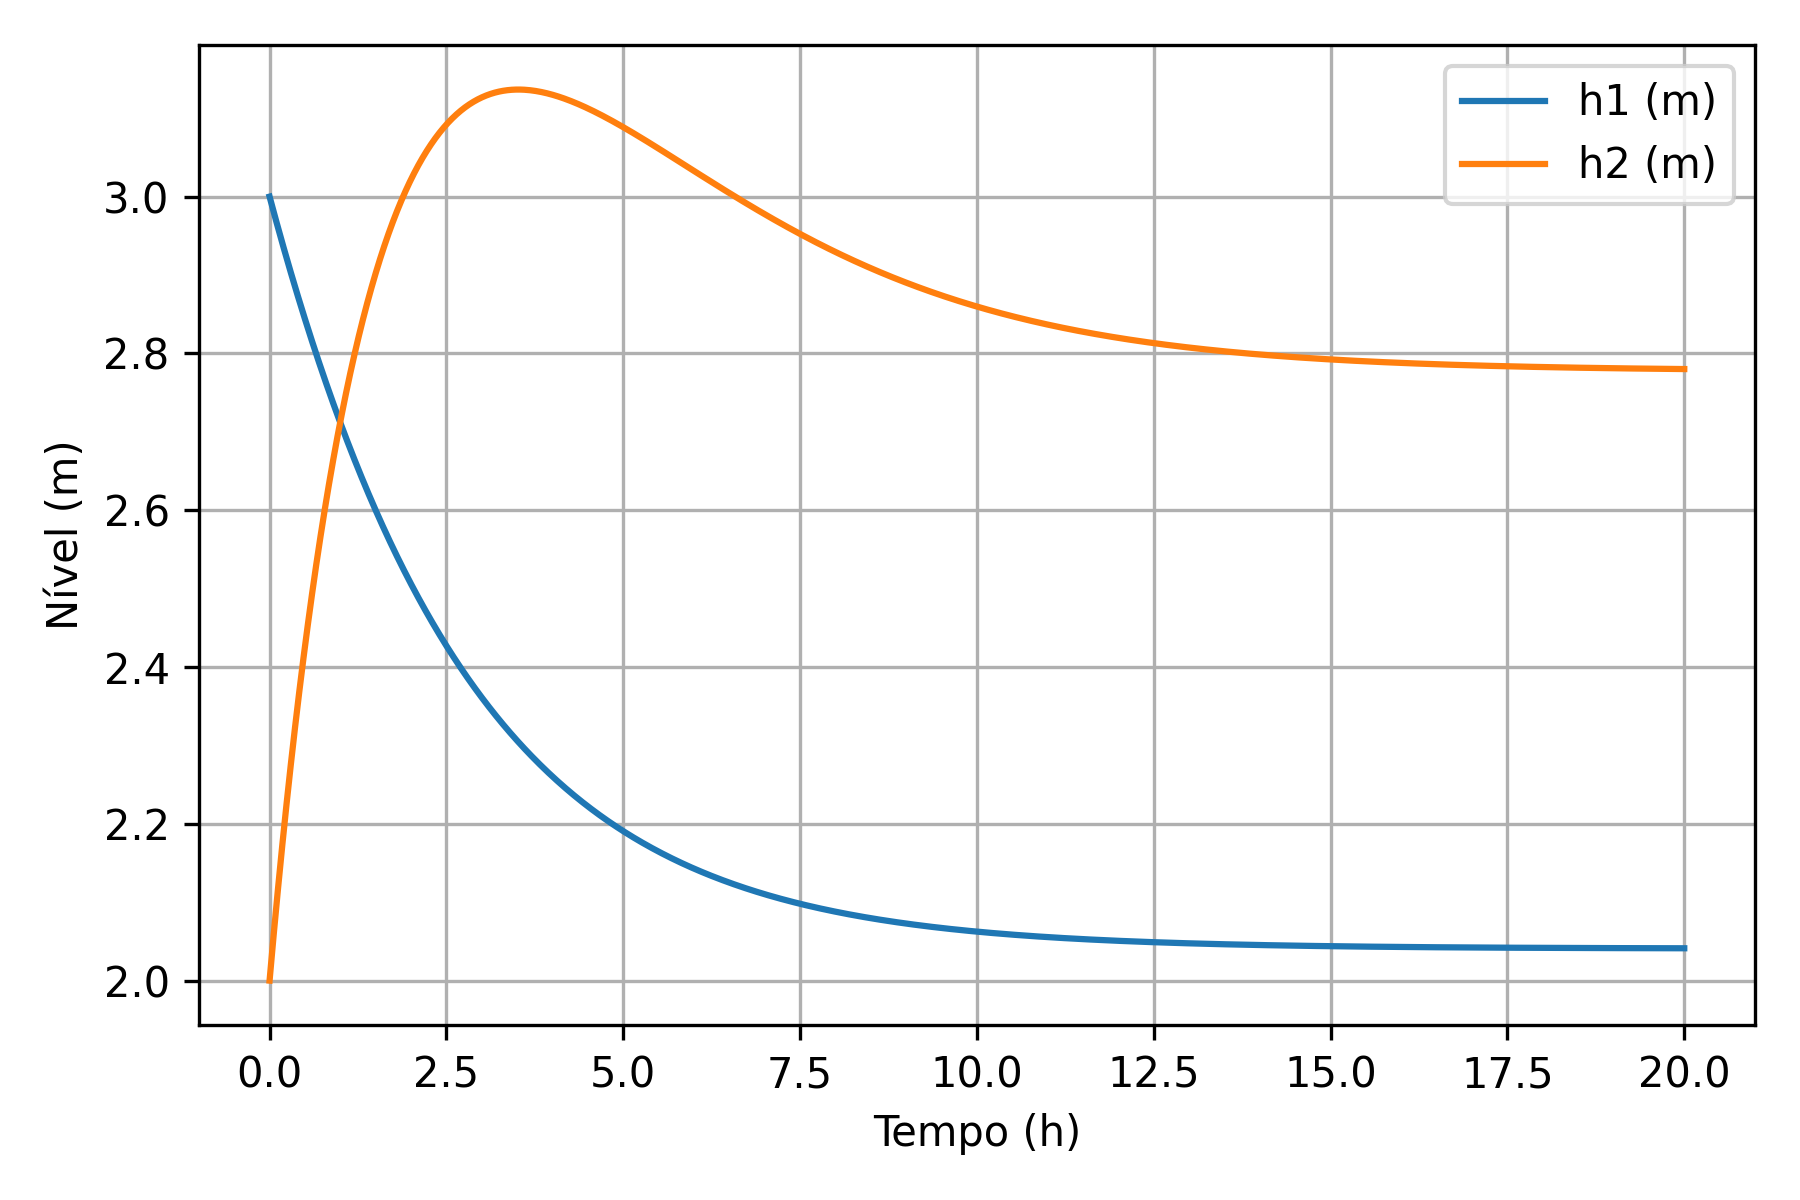
\includegraphics[width=0.7\textwidth]{figuras/questao1_niveis.png}
  \caption{Perfis temporais simulados dos níveis $h_1$ e $h_2$ durante 20 horas.}
  \label{fig:questao1}
\end{figure}
\begin{thebibliography}{9}
  \bibitem{referencia-exemplo}
  Autor, \emph{Título do Livro ou Artigo}, Editora, Ano.
\end{thebibliography}

\end{document}
